\chapter{Data Generation}
\label{chap:DataGeneration}
\par\noindent
\textit{\textbf{Introduction}} With the finished model, it is now possible to generate the actual data, via simulation. For this purpose, a matlab script initializes all relevant model parameters and feeds the simulation input, in this case the previously discussed track profile, into the model. 

\begin{figure}[H]
	\centering
	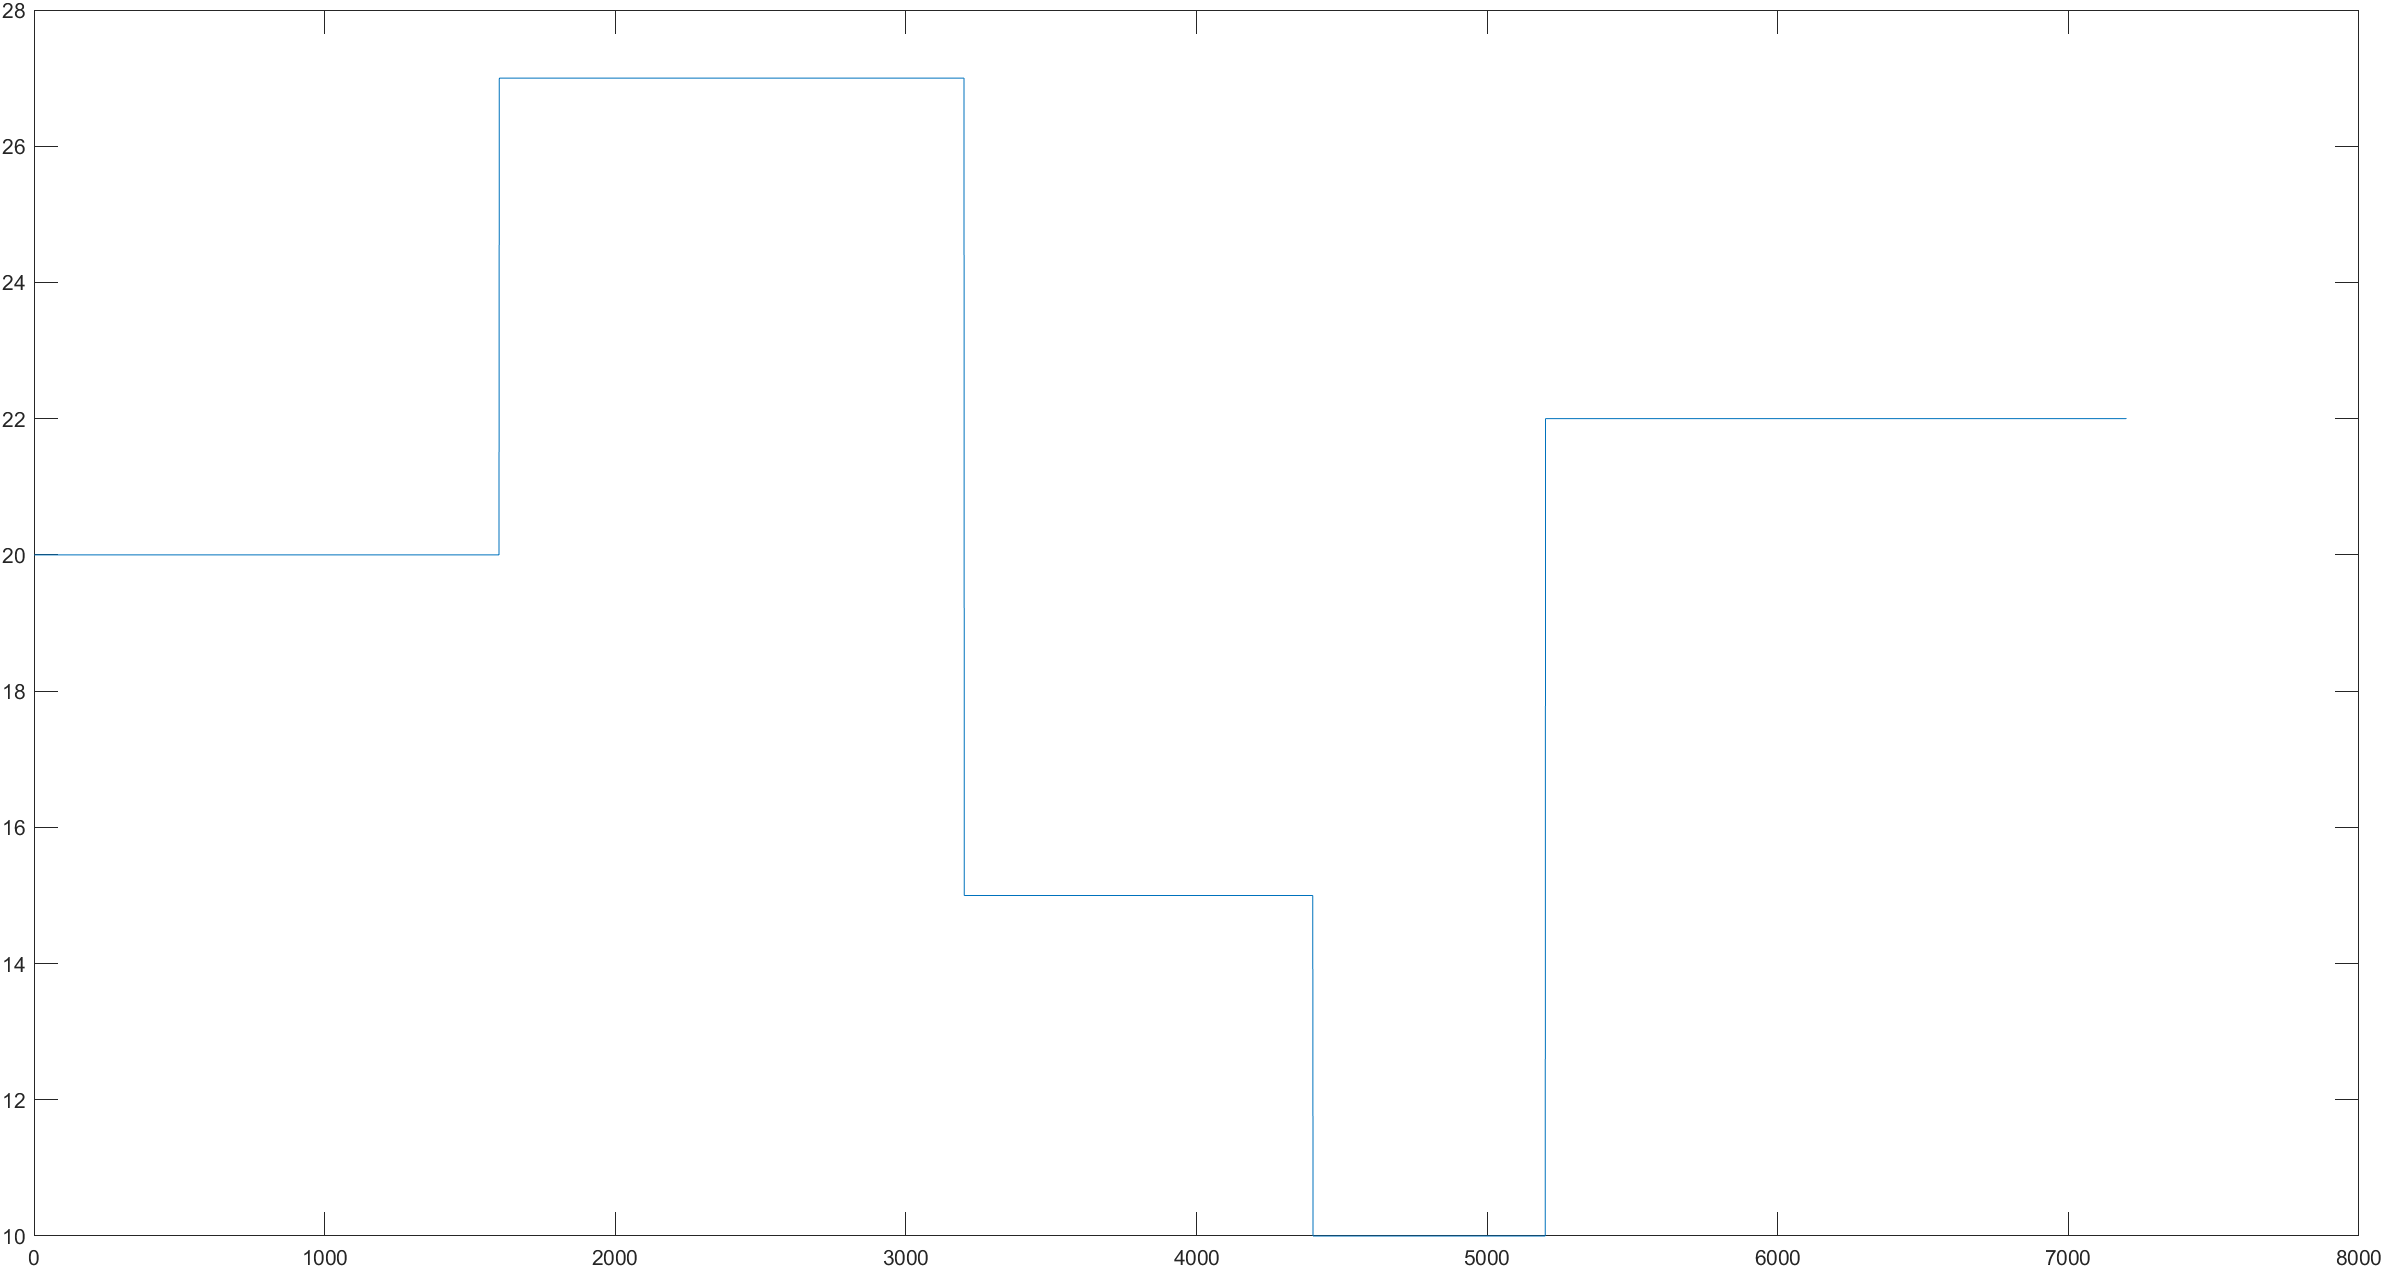
\includegraphics[width=\linewidth]{./pic/input}
	\caption{Simulation Input}
	\label{fig:siminput}
\end{figure}

\par\noindent
The track profile, as depicted above, basically describes at which time which maximum velocity is allowed, and thus the train either brakes or accelerates to match that value at all times. What we can gather from this is that the simulation is time-based. Here we have 7200 data points as in input, which is 3600 seconds times two for better precision.

\section{Matlab Code}
\label{sec:MatlabCode}
\par\noindent
We need to do some general configuration first, like clearing the workspace off all output which might still be present from previous simulations. 

\begin{lstlisting}
%% Initialise
clear all
clc
warning ('off','all');
numcores = 10; % configure number of cores to use in parallel processing
\end{lstlisting}

\par\noindent
We then need to initialise all constants which values remain the same for all simulations. Please refer to the code snippet below for descpriptions:

\begin{lstlisting}
%% Constants

RBD = 5; % regular operations pressure (bar)
VBD = 3.5; % full breaking pressure (bar)

l = 18; % wagon length (meters)
c = 250; % propagation velocity (km/h)

tf = 4; % brake cylinder filling time
tl = .1; 

p0 = 0; % initial pressure
Pres = 0/1000*[5.7/771 0 1.6]; % strahl formula for m/s velocity

alpha = 0.9; 

BPnum = [0.3 alpha]; 
BPden = [1 alpha]; 

%% Simulation input
tmax = 3600; % simulation time (seconds)
nmax = tmax * 2; % number of data points
t = linspace(0, tmax, nmax); % simulation time input
u = [20*ones(800*2,1); 27*ones(800*2,1); 15*ones(600*2,1); 10*ones(400*2,1); 
	22*ones(900*2,1); 0*ones(100*2,1)]; % track profile
simin.time = t; % set simulation time input
simin.signals.values = u; % set simulation signal input

trackgradient = 0; % pitch angle
\end{lstlisting}

\par\noindent
After having initialised all necessary constants, we now get to configuring variable simulation input.

\begin{lstlisting}
pool = readmatrix('pool.csv'); % read wagon pool
mkdir output; % make output directory

wagons = 1:1:40; % create array for number of wagons to loop over
friction = 0.05:0.01:0.78; % create array for friction coefficient to loop over
tracforce = 200000:1000:400000; % create array for traction force to loop over

track = 1; % counter to index input array for one batch of simulations
allruns = 1; % counter to keep track of total number of simulations completed

for i = length(tracforce):-1:1 		% all possible combinations of traction force,
	for j = length(friction):-1:1 	% friction coefficient and
		for k = length(wagons):-1:1 % number of wagons
			% save all previously initialised constans and sim input into
			% one array in
			in(track) = Simulink.SimulationInput('Simulation_v2');
			in(track) = in(track).setVariable('num_wagons',wagons(k));
			in(track) = in(track).setVariable('fc',friction(j));
			in(track) = in(track).setVariable('Ft',tracforce(i));
			
			in(track) = in(track).setVariable('alpha',alpha);
			in(track) = in(track).setVariable('BPden',BPden);
			in(track) = in(track).setVariable('BPnum',BPnum);
			in(track) = in(track).setVariable('c',c);
			in(track) = in(track).setVariable('l',l);
			in(track) = in(track).setVariable('nmax',nmax);
			in(track) = in(track).setVariable('p0',p0);
			in(track) = in(track).setVariable('pool',pool);
			in(track) = in(track).setVariable('Pres',Pres);
			in(track) = in(track).setVariable('RBD',RBD);
			in(track) = in(track).setVariable('simin',simin);
			in(track) = in(track).setVariable('t',t);
			in(track) = in(track).setVariable('tf',tf);
			in(track) = in(track).setVariable('tl',tl);
			in(track) = in(track).setVariable('tmax',tmax);
			in(track) = in(track).setVariable('trackgradient',trackgradient);
			in(track) = in(track).setVariable('u',u);
			in(track) = in(track).setVariable('VBD',VBD);
			
			% also save the respective values for traction force and
			% friction coefficient into arrays
			Ft(track) = tracforce(i);
			fc(track) = friction(j);
			
			track = track + 1;       
		end
	end
	
	fprintf('Starting pool for %d simulation runs.\n',length(in));
	parpool(numcores); % create a pool of #numcores workers for parallel processing
	out = parsim(in,'ShowProgress','on'); 	
	% start parallel simulations for all
	% entries of in, save output to out
											
	matrix = []; % create an empty matrix
	
	parfor l = 1:1:length(out) 	
	% parallel loop over out, which is an array that
	% holds all simulation outputs
	
		tmp = Write(l + allruns,out(l).get('velocity'),out(l).get('force')
			,out(l).get('pressure'),out(l).get('distance'),
			out(l).get('acceleration_neg'),out(l).get('ids'),t,u,
			trackgradient,Ft(l),fc(l)); % for each entry, pack all output into one single matrix
		matrix = [matrix;tmp]; % append to matrix
	end
	
	allruns = allruns + length(out); % update total number of simulations

	writematrix(matrix,'output/output.tsv','FileType','text','WriteMode','append',
		'Delimiter','tab'); 
	% write matrix, which holds all output matrices of the 
	% current batch, to a tsv file

	track = 1; % reset batch index 
	delete(gcp('nocreate')); % delete parallel pool
	fprintf('Run %d (of %d total) complete.\n',length(tracforce)-i,length(tracforce));
end
\end{lstlisting}

\par\noindent
As our aim is to generate large quantities of data, it becomes feasible to use use parallel processing for our simulations. For this purpose, we need to create an array to hold input for all simulation runs. There are three variables which change for each run, they are traction force of the locomotive, wheel/rail friction coefficient and number of wagons, respectively. A nested loop is used to create all possible combinations of these variables, and each single combination gets stored, as a new entry, in the array which holds all input.
\par
Variable ranges are from one to 40 for number of wagons, .05 to .78 for friction coefficient and 200000 to 400000 for traction force, with step sizes one, .01 and 1000 respectively. We therefore have a total number of $40*74*200 =  592000$ combinations. The obvious approach here would be to generate the full batch of 592000 input configurations, but performance and hardware limitations proved this to be unfeasible. Instead, we use rather small batche sizes of 2960 for parallel simulation.
\par
Writing of the output is also done in smaller batches. The best approach to minimize the number of file accessions is of course writing everything into one big matrix, thus storing in RAM, and then writing the matrix in one go. Unfortunately, growing an array by assignment or concatenation can be expensive. For large arrays, MATLAB must allocate a new block of memory and copy the older array contents to the new array as it makes each assignment. The other extreme would of course be to write every single output line directly, but the large number of file accessions required makes this even more unfeasible, so a middle ground is needed, and a batch size of ~3000 works relatively well, although this could surely be optimized with a bit of runtime analysis.
\par
The function below compresses all output of one single simulation into one matrix. Raw simulation output consists of a few time-series objects, like braking force and braking pressure, as well as some metadata. These objects are fed into the write function, which does as many loops as there are rows in the time-series objects. It then packs all rows from each time-series into one big row, adds the meta-data and appends the large row to the matrix, which gets returned at the end. Refer to section \ref{sec:DataStructure} for a more detailed look at the structure of the output matrix.

\begin{lstlisting}
function ret = Write(id,velocity,force,pressure,distance,acceleration,wagon_ids,t,u,grad,ft,fc)
	numrows = get(force,'Length');
	wagon_ids = double(wagon_ids);
	time = force.Time;
	matrix = [];
	
	for i = 1:1:numrows
		f = getdatasamples(force,i);
		p = getdatasamples(pressure,i);
		v = getdatasamples(velocity,i);
		a = getdatasamples(acceleration,i);
		d = getdatasamples(distance,i);
		
		row = [id,time(i),f,p,v,a,d,wagon_ids,grad,ft,fc]; 	% TODO: add simulation input aka track profile to matrix
		%		print wagon ids as list delimited by colon (,)
		%		performance?
		matrix = [matrix;row];
	end
	fprintf('Created output matrix for simid %d\n',id);
	% writematrix(matrix,'output/output.tsv','FileType','text','WriteMode','append','Delimiter','tab');
	% ret = 1;
	% fprintf('Create output matrix for Simulation ID %d\n', id);
	ret = matrix;
end
\end{lstlisting}

\begin{lstlisting}[language=python]
import csv
import random

with open('pool.csv', 'w', newline='') as pool:
	fieldnames = ['Wagon_ID', 'Mass', 'Braking_eff']
	writer = csv.DictWriter(pool, fieldnames=fieldnames)
	
	writer.writeheader()
	for i in range(0,500): # create 500 randomized wagons
		mass = random.randrange(12000, 90000, 100) # create random wagon mass between 12 t and 90 t with step size 100
		braking_eff = round(random.uniform(0.75, 0.95),2) # create random braking efficiency as uniform distribution between 75 % and 95 %
		writer.writerow({'Wagon_ID': i, 'Mass': mass, 'Braking_eff': braking_eff})
\end{lstlisting}

\par\noindent
The above python script is used to create a randomized pool of 500 wagons to be used in simulation. Each wagon has a unique id, a randomized mass, ranging between 12000 and 90000 kilograms, and a braking efficiency, which is a uniform distribution between .75 and .95.

\section{Data Structure}
\label{sec:DataStructure}
\par\noindent
As has been denoted previously, generated data should be suitable for big data processing. The first approach was to create a new directory for each iteration, and also save the different parameters to different files. Since this is very inefficient in terms of number of file accessions and therefore negatively impacts performance, as well as being unsuitable for transformations to big data file systems like Apache Hadoop or Apache Hive, it has been proposed to write all output into one single file. Let's take a look at the structure first.

\begin{tabular}{|c|c|c|c|c|c|c|c|c|c|c|c|c|c|c|c|c|}
	\hline
	simID & Timestamp & $F_{wagon0}$ & ... & $P_{wagon0}$ & ... & $v_{wagon0}$ & ... & $a_{wagon0}$ & ... & Distance & Wagons & Track angle (tentative) & $F_{t}$ & fc & Track profile \\
	\hline
	&  &  &  &  &  &  &  &  &  &  &  &  &  &  &  &  \\
	\hline
	&  &  &  &  &  &  &  &  &  &  &  &  &  &  &  &  \\
	\hline
	&  &  &  &  &  &  &  &  &  &  &  &  &  &  &  &  \\
	\hline
	&  &  &  &  &  &  &  &  &  &  &  &  &  &  &  &  \\
	\hline
	&  &  &  &  &  &  &  &  &  &  &  &  &  &  &  &  \\
	\hline
	&  &  &  &  &  &  &  &  &  &  &  &  &  &  &  &  \\
	\hline
\end{tabular}

\par\noindent
Some output objects are time-series, namely braking force, braking pressure, acceleration, distance and velocity. Force, pressure and acceleration, which get measured for every wagon, look like this

\begin{tabular}{|c|c|c|c|c|}
	\hline
	Timestamp & $Wagon_{1}$ & $Wagon_{2}$ & ... & $Wagon_{40}$ \\
	\hline
	0 & 0 & 0 & 0 & 0 \\
	\hline
	10 & $x_{1}$ & $x_{2}$ & ... & $x_{40}$ \\
	\hline
	... & ... & ... & ... & ... \\
	\hline
	3600 & $y_{1}$ & $y_{2}$ & ... & $y_{40}$ \\
	\hline
\end{tabular}

\par\noindent
whereas distance and velocity only have two columns and thus look like this

\begin{tabular}{|c|c|}
	\hline
	Timestamp & Value \\
	\hline
	0 & 0 \\
	\hline
	.. & .. \\
	\hline
	3600 & $x$ \\
	\hline
\end{tabular}

\par\noindent
Since they all posses the same number of lines, which is the number of timestamps at which measurements were taken, all columns from all these objects may be compressed into a single table. All columns containing meta-information, for example simulation id, which theoretically only needs to be printed once, get filled with the same value for all lines, and since the number of wagons may vary from one to 40, all possibly empty columns get filled with zeros, so that we do not get any columns containing no value. 

\section{Analysis of generated Data}
\label{sec:AnalysisOfGeneratedData}